\chapter{浮游生物特征分析}
\label{cha:phy}

在浮游生物分类过程中,特征分析是一个重要环节,得到特征的好坏会直接影响分类的最终结果。我们对浮游生物特征进行分析,根据浮游生物形态特征,从各个角度选取适合的特征提取方法进行特征描述,然后从获得的特征中选取有效的特征子集。本章主要介绍对浮游生物形态特征进行提取的方法,以及去除特征中冗余信息采用的特征选择算法。


\section{浮游生物特征提取}
\label{sec:FeatureExtraction}

人们在识别浮游生物过程中,会根据浮游生物的形状、纹理等特征对浮游生物进区分。浮游生物自动分类识别系统正是模拟人类对浮游生物分类识别的过程进行设计的,因此选择特征提取方法时可以结合人类在识别浮游生物时采用的特征。在本文中,根据浮游生物的形态特征,并结合经典计算机视觉算法对浮游生物特征进行提取,主要使用的方法有以下几种:几何灰度特征;粒子测度;纹理特征,包括变差函数、Gabor滤波器、二元梯度轮廓、局部二值模式;局部特征,包括方向梯度直方图、内距离形状上下文、尺度不变特征变换。

\subsection{几何和灰度特征}
\label{sec:graphs}

目标的几何灰度为浮游生物的基本特征,简单的几何和灰度(例如面积、周长、灰度对比度等)等统计标量可以用来表示浮游生物的形态特征。在本文的研究中,共使用43个几何和灰度特征对浮游生物进行描述,下面介绍其中部分特征。

\textbf{几何标量特征:}

\begin{enumerate}
\item 周长:为图像中包围目标的轮廓边缘上所有像素数量之和。
  \begin{eqnarray}
  L = \sum^{M}_{x=1}\sum^{N}_{y=1}n(x,y)
  \end{eqnarray}
  其中,$L$表示周长,$x,y$为像素点坐标,$n(x,y)$表示物体的边缘二值图,$M,N$为图像高和宽。
\item 面积:是指图像中目标区域内像素数量之和。
  \begin{eqnarray}
  A = \sum^{M}_{x=1}\sum^{N}_{y=1}f(x,y)
  \end{eqnarray}
  其中,$A$为面积,$f(x,y)$代表目标的二值图。
\item 体态比:表示可以包围目标的最小外接矩形的长和宽之比。
  \begin{eqnarray}
  C = \frac{W}{H}
  \end{eqnarray}
  其中,$C$为体态比,$W,H$为最小外接矩形的长宽。
\item 圆形度:表示目标区域的圆形程度。
  \begin{eqnarray}
  e = \frac{4\pi A}{L \times L}
  \end{eqnarray}
  其中,$e$表示圆形度,当$e$等于1时目标的形状为圆形,$e$越小表示目标的形状越不规律,形状与圆形差距较大。
\item 伸长率:是指可以拟合目标形状的最优椭圆的长轴和短轴之比。
  \begin{eqnarray}
  \delta = \frac{Major}{Minor}
  \end{eqnarray}
  其中,$\delta$表示伸长率,$Major$表示椭圆的长轴,$Minor$表示短轴。
\item 凸率:是指目标物体的面积与目标物体的凸壳面积之间的比值。
  \begin{eqnarray}
  C_{R} = \frac{A}{\sum^{M}_{x=1}\sum^{N}_{y=1}k(x,y)}
  \end{eqnarray}
  其中,$C_R$为凸率,$k(x,y)=\left\{ \begin{array}{ll} 1 & (x,y)\in \textrm{目标区域凸包部分}\\ 0 & (x,y)\notin \textrm{目标区域凸包部分} \end{array} \right.$。
\item 等效球直径:是指与目标物体体积相同的球的直径。
  \begin{eqnarray}
  Esc = 2 \times \sqrt{\frac{A}{\pi}}
  \end{eqnarray}
\item 最大费雷特直径:弗雷特直径是一种粒径表示方法,沿着一定方向可以测量获得的投影目标区域轮廓两边界平行线间的距离。最大弗雷特直径即目标物体轮廓边界上两平行线间距离的最大值。
\end{enumerate}

\textbf{灰度标量特征:}
\begin{enumerate}
\item 最小值:是指目标范围中全部像素点的最小灰度值。
  \begin{eqnarray}
  I_{min} = \min_{I}I(x,y)
  \end{eqnarray}
  其中,$I$表示灰度图像,$x,y$表示图像中像素点的坐标。
\item 最大值:是指目标范围中全部像素点的最大灰度值。
  \begin{eqnarray}
  I_{max}=\max_{I}I(x,y)
  \end{eqnarray}
\item 平均值:是指目标范围中全部像素点灰度值的均值。
  \begin{eqnarray}
  I_{arg} = \frac{\sum_{I}I(x,y)}{A}
  \end{eqnarray}
\item 总密度:是指目标范围中所有像素点灰度值之和。
  \begin{eqnarray}
  I_{den}=\sum_{I}I(x,y)
  \end{eqnarray}
\item 标准差:是指目标范围中灰度值的标准差。
  \begin{eqnarray}
  I_{\sigma} = \sqrt{\frac{1}{A}\sum_{I}(I(x,y)-I_{arg})^{2}}
  \end{eqnarray}
\item 对比度:表示目标区域中最亮和最暗像素区域的对比程度。
  \begin{eqnarray}
  CON = \sum^{k}_{x=1}\sum^{k}_{y=1}{G(x,y)}^2
  \end{eqnarray}
  其中,$G$表示目标图像的灰度共生矩阵,$k$表示目标图像中灰度值级数。
\item 自相关:反映目标区域中纹理的一致性。
  \begin{eqnarray}
  COR = \sum^{k}_{x=1}\sum^{k}_{y=1}\frac{xyG(x,y)-u_{x}u_{y}}{s_{x}s_{y}}
  \end{eqnarray}
  其中
  \begin{eqnarray}
  u_{x}=\sum^{k}_{x=1}\sum^{k}_{y} x G(x,y),  ~~~~  u_{y}=\sum^{k}_{x=1}\sum^{k}_{y=1} y G(x,y)
  \end{eqnarray}
  \begin{eqnarray}
  s^{2}_{x}=\sum^{k}_{x=1}\sum^{k}_{y=1}G(x,y)(x-u_{y})^{2},  ~~~~   s^{2}_{y}=\sum^{k}_{x=1}\sum^{k}_{y=1}G(x,y)(y-u_{y})^{2}
  \end{eqnarray}
\item 熵:是图像中所具有信息量的度量。
  \begin{eqnarray}
  ENT = -\sum^{k}_{x=1}\sum^{k}_{y=1}G(x,y)\log G(x,y)
  \end{eqnarray}
\end{enumerate}

除了上述几种几何和灰度特征以外,在本文还使用了不变矩、对称性等标量值来描述浮游生物的基本形态特征。

\subsection{粒子测度}

粒子测度(Granulometry)由Matheron等人在1978年提出~\cite{matheron1978randoms},可以用来计算二值图像中目标区域的大小分布情况。粒子测度的基本思想是对二值图做开运算,在开运算过程中不断增加结构元素的大小,并记录下在此过程中图像中区域内像素数量的变化。
\begin{eqnarray}
G\circ T = \cup\{T+x : T+x \subset G \}
\end{eqnarray}
\begin{eqnarray}
\psi_{\lambda}(G) = G\circ\lambda T
\end{eqnarray}

其中G为二值图,T为结构元素,$\circ$为开运算,$\lambda$为一个正数变量,表示进行开运算的次数,$\psi_{\lambda}(G)$表示经过开运算后得到的二值图像。
\begin{eqnarray}
F_{G}(\lambda) = 1-\frac{v(\psi_{\lambda}(G))}{v(G)}
\end{eqnarray}

其中$v(G)$表示得到原始图像中目标区域的像素数量,$F_{G}(\lambda)$为粒子分布,它可以描述图像中目标的区域分布特征。

在本文采用粒子测度提取浮游生物的特征,在实验中设置了两组参数,分别采用不同变换的结构元素进行开运算。第一组参数是将结构元素大小由2变到50,间隔为4,记录下图像中目标区域像素数量的变化情况。第二组参数是将结构元素大小由5变到60,间隔为5,记录图像中像素数量的变化。

\subsection{纹理特征}

\subsubsection{变差函数}

变差函数(Variogram)是Motheron在1965年提出的一种矩估计方法,可以表示区域化变量的随机性,反应了区域化变量在某个方向上某一距离范围内的相关程度。从描述纹理特征的角度来考虑,图像中浮游生物的灰度值可以看成反应图像纹理的随机性和相关程度的区域化变量~\cite{曹健渭2010基于散斑纹理变差函数的平磨表面粗糙度测量技术},因此用变差函数能够有效表示图像的纹理特性,具体形式如下:
\begin{eqnarray}
\gamma(h) = \frac{1}{2N(h)}\sum^{N(h)}_{i=1}[Z(x)-Z(x+h)]^{2}
\end{eqnarray}

其中$h$是两个像素之间沿着某一方向的距离,$N(h)$是指在一定的区域内像素间距离为h的对数,$Z(x)$和$Z(x+h)$为点$x$和$x+h$的灰度值。用变差函数描述纹理特征时,选用一定的窗口、步长和方向计算函数值,然后取平均值赋给窗口中心点,得到差变函数纹理图。

\subsubsection{Gabor滤波器}
\label{sec:multifig}

Gabor滤波器是一种基于信号处理的纹理分析方法,其实质是一种加了高斯窗口的傅里叶变换,通过窗口的变化可以提取图像不同尺度和不同位置上的纹理信息。Gabor变换符合人和动物的视觉机理,具有良好的方向选择性和空间局部性~\cite{高梓瑞2012gabor},可以精确的描述局部纹理特性,因此该方法被广泛的用来提取纹理特征。本文中使用二维Gabor滤波器来描述浮游生物的纹理特征。

二维Gabor滤波器的冲击响应为~\cite{王铌2006海洋浮游生物数字图像处理方法}:
\begin{eqnarray}
h(x,y) = \frac{1}{2\pi \sigma^{2}} e^{-\frac{x^{2}+y^{2}}{2\sigma^{2}}+2\pi jF(x\cos\theta+y\sin\theta)}
\end{eqnarray}
其中$\theta$为方向,$F$为中心频率,这两个参数决定着Gabor滤波器的位置,即改变这两个参数可以得到不同滤波通道。Gabor滤波器的本质就是与原图像进行卷积,即
\begin{eqnarray}
Q(x,y)=I(x,y)*h(x,y)
\end{eqnarray}
其中$I(x,y)$为原图像,$Q(x,y)$为Gabor滤波的结果。采用不同参数卷积后会得到不同的输出图像,每幅输出图像的均值和标准差可以表示该图像的纹理特性,所有图像的值可以组成一个特征向量来描述原始图像的纹理特征。
\begin{eqnarray}
mean = \frac{\sum^{n-1}_{x=0}\sum^{m-1}_{y=0}Q(x,y)}{m \times n}
\end{eqnarray}
\begin{eqnarray}
std=\sqrt{\frac{\sum^{n-1}_{x=0}\sum^{m-1}_{y=0}[Q(x,y)-mean]^{2}}{m \times n}}
\end{eqnarray}
其中$m, n$表示图像的长和宽,mean和std分别为卷积后图像的均值和标准差。若在实验中参数选用a个方向,b个中心频率,那么一共会得到$a \times b$个不同的Gabor滤波器,从而获得$a \times b$张图像。然后分别计算每张滤波后得到图像的均值和标准差,将获得$a \times b \times 2$个值组成一个特征向量,该向量可以有效的描述目标图像的纹理特征。在本文实验中,我们为Gabor滤波器选定了不同的参数,包括6个频率、8个方向,如图~\ref{fig:gabor}。用Gabor滤波器提取特征时,每幅图像会获得一个96($6 \times 8 \times 2$)维的特征向量。
\begin{figure}[H] % use float package if you want it here
  \centering
  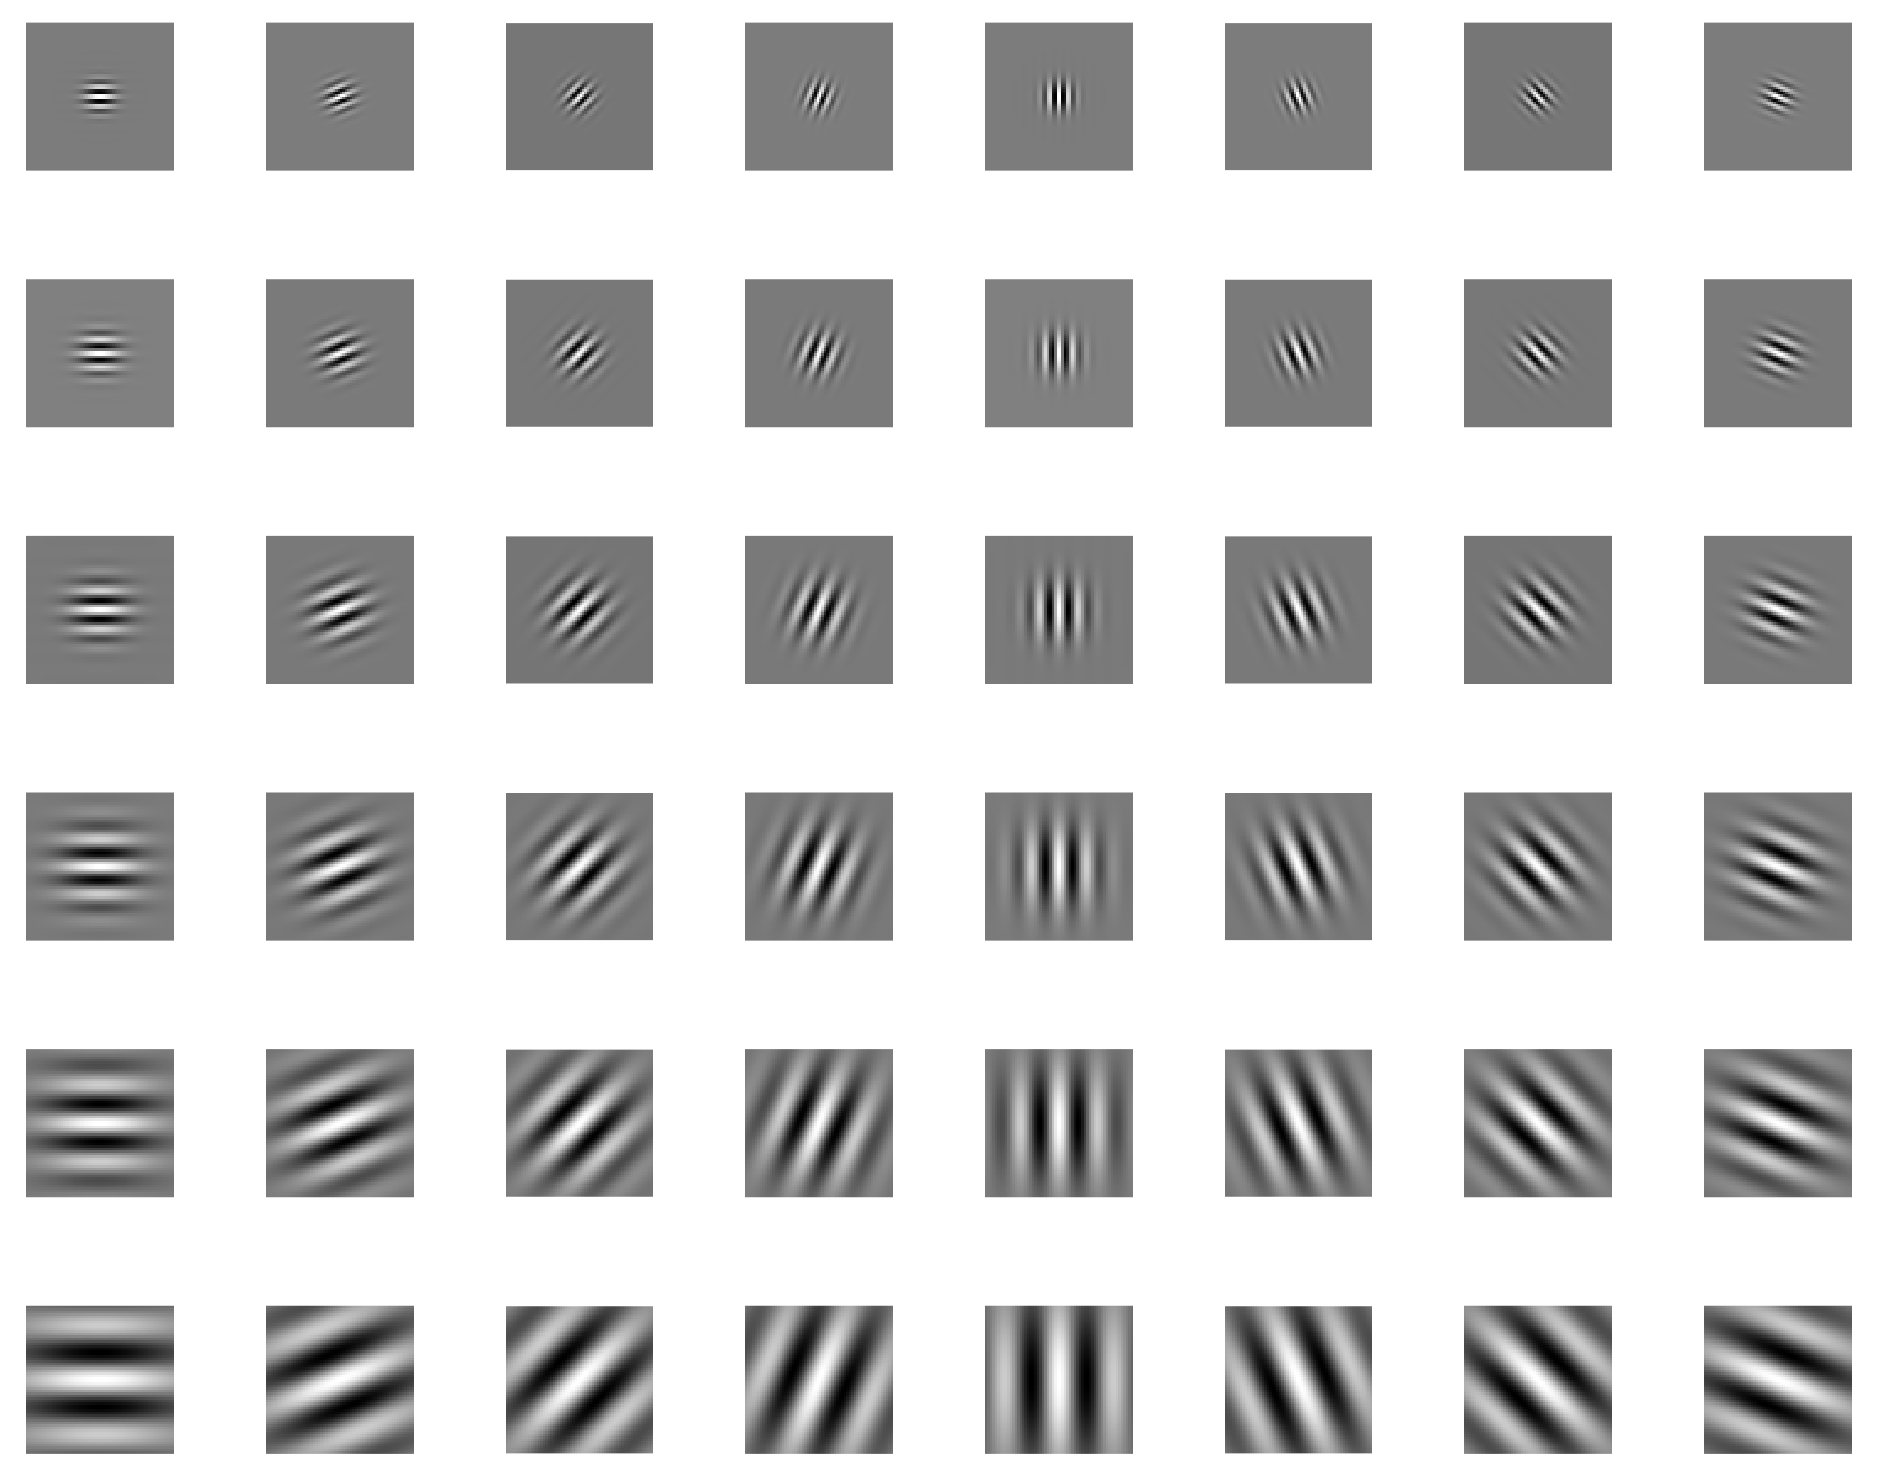
\includegraphics[height=7cm]{Gabor/gabor}
  \caption{不同参数下的Gabor滤波器}
  \label{fig:gabor}
\end{figure}

\subsubsection{局部二值模式}

局部二值模式(Local Binary Pattern, LBP)由Timo Objala等人在1994年提出~\cite{ojala1994performance},它是一种描述图像纹理特征的方法,该算法有灰度不变性和旋转不变性。局部二值模式的基本思想是用LBP值描述目标中每一个像素与其邻域像素之间的差别,然后通过统计整幅图像中的LBP值出现的频率来描述图像的特征。

通常LBP算子以每个像素点的$3 \times 3$邻域为窗口,假设中心点的灰度值为$g_{c}$,邻域点的值为$g_{0},g_{1},\dots,g_{7}$,则该区域内灰度值的联合分布可以表示为:
\begin{eqnarray}
T=t(g_{c},g_{0},\cdots,g_{7})
\end{eqnarray}

在计算图像中每一个像素点的LBP值时,将该点的灰度值作为阈值,$3 \times 3$邻域内另外8个点的灰度值分别与阈值比较,即:
\begin{eqnarray}
T=t(g_{c},g_{0}-g_{c},\cdots,g_{7}-g_{c})
\end{eqnarray}
由于联合分布$T$的取值比较广范,不利于描述,因此将灰度做差的结果用两个值来表示,即若中心阈值与其邻域像素点的灰度值之差值为负数,则将邻域中该点值记为0,否则记为1:
\begin{eqnarray}
T\approx t(s(g_{0}-g_{c}),s(g_{1}-g_{c}),\cdots,s(g_{7-g_{c}}))
\end{eqnarray}
其中$s$为符号函数,即$s(x)=\left \{ \begin{array}{ll} 1 & x>0\\ 0 & x<0 \end{array}\right.$。

给每个像素点乘以一个权值$2^{i}$并求和,就可以得到中心点周围区域纹理的描述值,称为LBP值,计算方法为:
\begin{eqnarray}
LBP_{8} = \sum^{7}_{i=0}s(g_{i}-g_{c})2^{i}
\end{eqnarray}

图~\ref{fig:lbpvalue}为LBP描述子的计算过程。
\begin{figure}[H] % use float package if you want it here
  \centering
  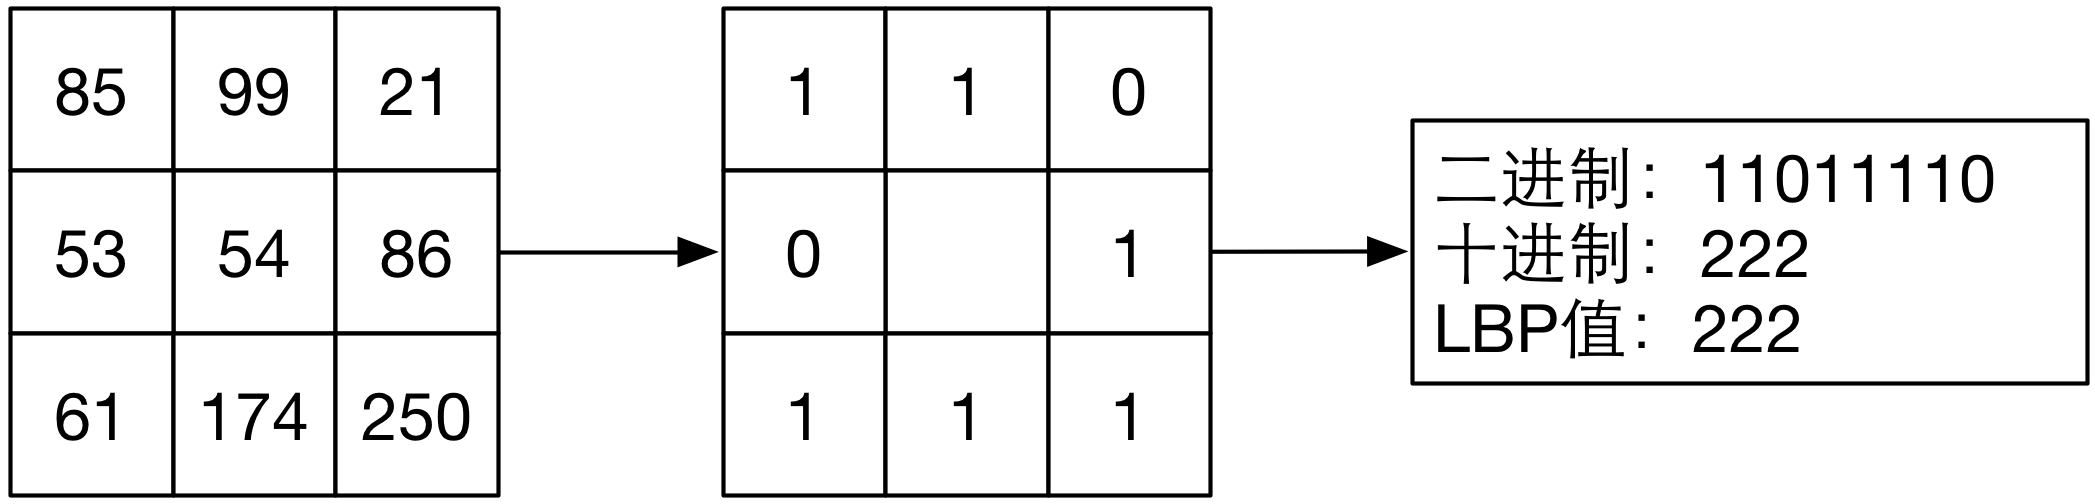
\includegraphics[height=2.5cm]{LBP/lbpvalue}
  \caption{计算LBP值}
  \label{fig:lbpvalue}
\end{figure}

经过上述过程后就能够得到图像中所有像素点的LBP值,然后用直方图统计图像中LBP值的出现频率,用其描述目标图像的纹理特征。综上采用LBP算法提取图像纹理特征的基本过程如下(如图~\ref{fig:lbpframework}):
\begin{figure}[H] % use float package if you want it here
  \centering
  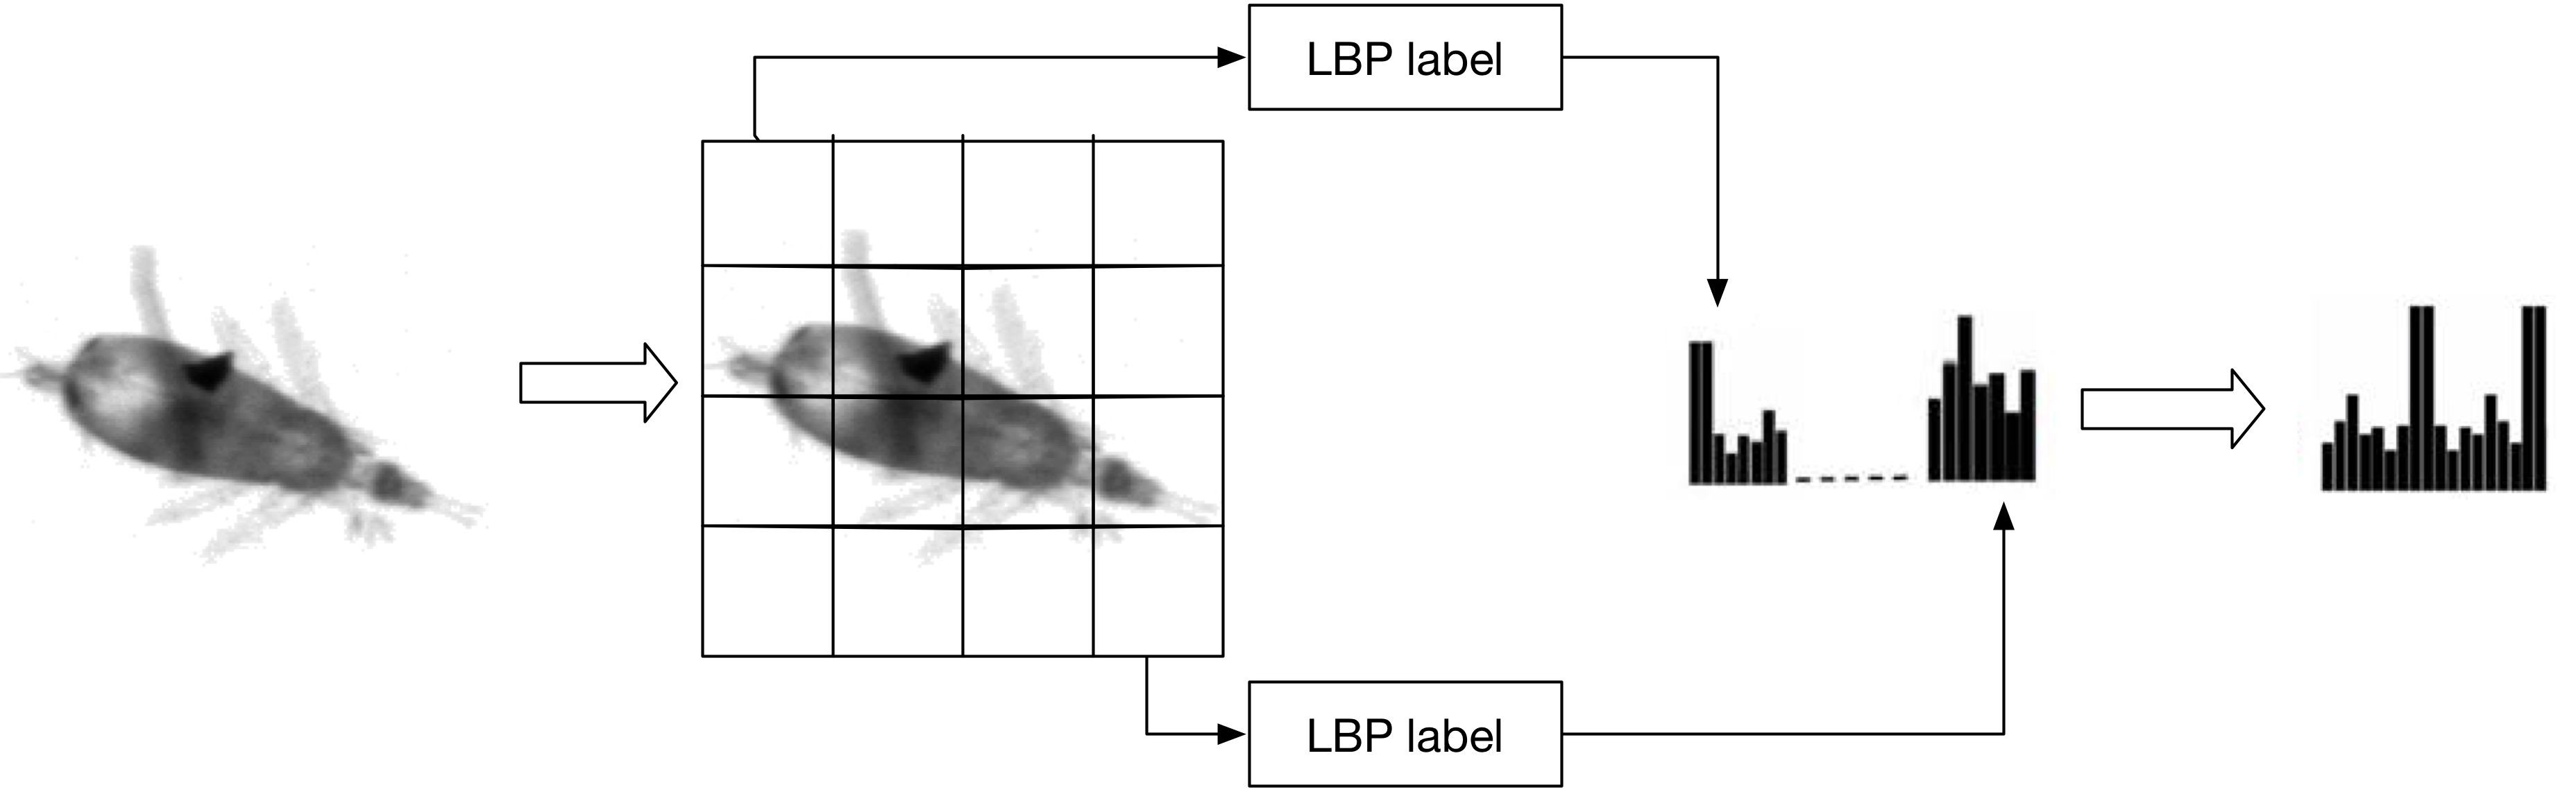
\includegraphics[height=4.5cm]{LBP/lbpframework}
  \caption{LBP特征提取过程}
  \label{fig:lbpframework}
\end{figure}
\begin{enumerate}
\item 先将图像分为多个子区域。
\item 分别计算子区域中每个像素点的LBP值。
\item 用直方图分别统计每个子区域内LBP值的出现频率,对每个子区域内的纹理特征进行描述。
\item 将一幅图像中全部子区域的直方图串联到一起,就可以得到描述该幅图像的LBP特征向量。
\end{enumerate}

\subsubsection{二元梯度轮廓}

二元梯度轮廓(Binary Gradient Contours, BGC)由Fernandez等人在2011年提出~\cite{fernandez2011image},是一种纹理特征描述算子。二元梯度轮廓与局部二值模式相似,它的基本思想是用BGC值对图像中每个像素与其$3 \times 3$邻域内像素梯度的差别进行描述,通过直方图统计BGC值的出现频率来描述图像的纹理特征。

二元梯度轮廓与局部二值模式的不同之处在于,二元梯度轮廓沿一定封闭路径计算中心像素的8邻域像素之间的梯度,然后使用0作为阈值,若两像素间梯度值大于0则记为1,否则记为0。在这个过程中,计算梯度的路径有多种,其中典型的三种路径如图~\ref{fig:BGCpath}所示。
\begin{figure}[h]
  \centering%
  \subcaptionbox{单程二元梯度轮廓\label{fig:BGC1}}%标题的长度,超过则会换行,如下一个小图。
    {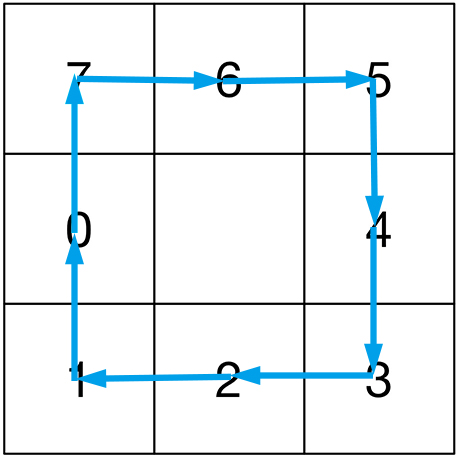
\includegraphics[height=3cm]{BGC/BGC1}}%
  \hspace{4em}%
  \subcaptionbox{双程二元梯度轮廓\label{fig:BGC2}}
      {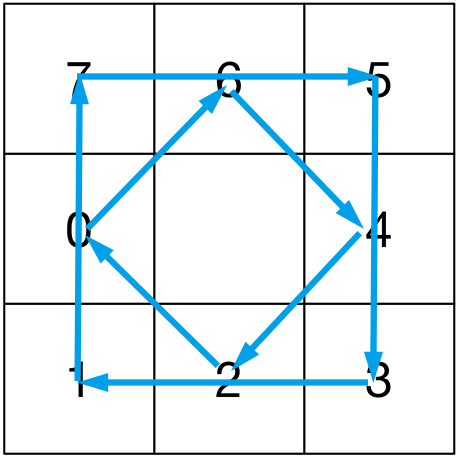
\includegraphics[height=3cm]{BGC/BGC2}}
  \hspace{4em}%
  \subcaptionbox{三程二元梯度轮廓\label{fig:BGC3}}
      {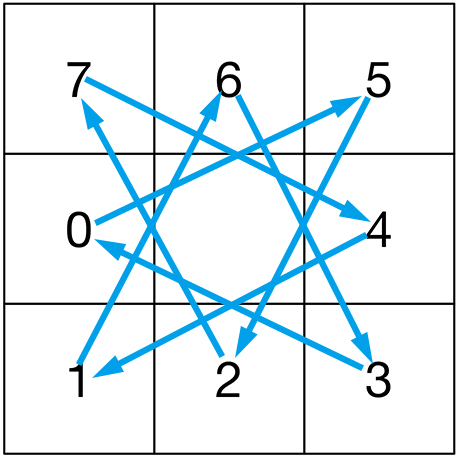
\includegraphics[height=3cm]{BGC/BGC3}}
  \caption{二元梯度轮廓的路径}
  \label{fig:BGCpath}
\end{figure}

图~\ref{fig:BGC1}由一条路径构成,叫做单程二元梯度轮廓(BGC1),公式如下:
\begin{eqnarray}
g_{1}=\left[ \begin{array}{l} s(I_{7}-I_{0}) \\ s(I_{6}-I_{7}) \\ s(I_{5}-I_{6}) \\ s(I_{4}-I_{5})\\ s(I_{3}-I_{4})\\ s(I_{2}-I_{3})\\ s(I_{1}-I_{2})\\ s(I_{0}-I_{1}) \end{array} \right]
\end{eqnarray}

图~\ref{fig:BGC2}中有两条路径,叫做双程二元梯度轮廓(BGC2),将两个回路计算的结果连接在一起来共同来表示每一个点:
\begin{eqnarray}
g_{2_{1}}=\left[ \begin{array}{l} s(I_{6}-I_{0})\\ s(I_{4}-I_{6})\\ s(I_{2}-I_{4})\\ s(I_{0}-I_{2}) \end{array} \right] , ~~~ g_{2_{2}}=\left[ \begin{array}{l} s(I_{7}-I_{1})\\ s(I_{5}-I_{7})\\ s(I_{3}-I_{5})\\ s(I_{1}-I_{3}) \end{array} \right]
\end{eqnarray}
\begin{eqnarray}
g_{2}=\left[ \begin{array}{l} g_{2_{1}}\\ g_{2_{2}} \end{array} \right]
\end{eqnarray}

同样,图~\ref{fig:BGC3}叫做三程二元梯度轮廓(BGC3),其表达式为:
\begin{eqnarray}
g_{3}=\left[ \begin{array}{l} s(I_{5}-I_{0})\\ s(I_{2}-I_{5})\\ s(I_{7}-I_{2})\\ s(I_{4}-I_{7})\\ s(I_{1}-I_{4})\\ s(I_{6}-I_{1})\\ s(I_{3}-I_{6})\\ s(I_{0}-I_{3}) \end{array} \right]
\end{eqnarray}

因此每个像素都可以获得一个8位二进制二元梯度轮廓值,求取图像点的各种二元梯度轮廓值的公式如下:
\begin{eqnarray}
BGC_{1} = w^{T}_{8}g_{1}-1\\
BGC_{2} = 15w^{T}_{4}g_{2_{2}}+w^{T}_{4}g_{2_{1}}-16\\
BGC_{3} = w^{T}_{8}g_{3}-1
\end{eqnarray}
其中,$w^{T}_{j}=[2^{j-1}  2^{j-2}  \dots  2^{1} 2^{0}]$。

根据以上式子可以求出图像中每个像素点的二元梯度轮廓值,然后用直方图统计图像中二元梯度轮廓值的出现频率。

\subsection{局部特征}

\subsubsection{内距离形状上下文}
\label{sec:onefig}

内距离形状上下文(Inner-Distance Shape Context, IDSC)由凌海滨在2007年提出~\cite{ling2007shape},它是对形状上下文方法(Shape Context, SC)~\cite{belongie2002shape}的一种改进。形状上下文是一种描述目标形状特征的方法,在2002年由Serge Belongie等人提出,该方法通过考察目标物体边缘上的点之间的空间位置关系来描述目标的形状特征,具体实现过程如下。

\begin{enumerate}
\item 首先提取目标物体(如图~\ref{fig:a})的轮廓边缘(如图~\ref{fig:a-edge})。由于轮廓上的像素点较多,需要从中采样n个点$P=\{p_1,\dots,p_n\}$来近似表示目标物体的轮廓(如图~\ref{fig:a-point})。在采集这n个点时要尽量保证采样点的重心和目标物体重心重合。
  \begin{figure}[H]
  \begin{minipage}{0.33\textwidth}
    \centering
    
\includegraphics[height=3cm]{IDSC/a}
    \caption{目标图像}
    \label{fig:a}
  \end{minipage}\hfill
  \begin{minipage}{0.33\textwidth}
    \centering
    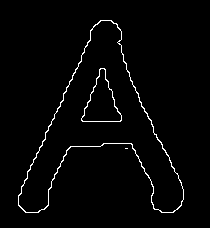
\includegraphics[height=3cm]{IDSC/a-edge}
    \caption{轮廓边缘}
    \label{fig:a-edge}
  \end{minipage}
  \begin{minipage}{0.33\textwidth}
    \centering
    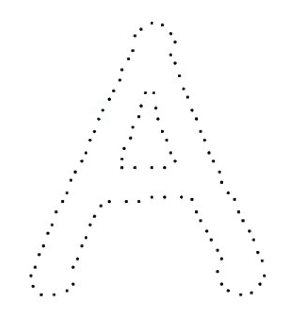
\includegraphics[height=3cm]{IDSC/a-point}
    \caption{采样点}
    \label{fig:a-point}
  \end{minipage}
  \end{figure}
\item 假设图~\ref{fig:a-point}中第i个采样点为$p_{i}$,则连接这个采样点$p_i$与其他$n-1$个点可以构成$n-1$个向量,这些向量可以表示该点$p_i$与轮廓上其他点间的相对位置关系。以$p_{i}$为原点建立对数极坐标系,如图~\ref{fig:a-log}所示,将图像中的坐标变换为极坐标,公式如下:
\begin{eqnarray}
r=\sqrt{(x-x_{0})^{2}+(y-y_{0})^{2}}, ~~~ \theta=arctan(\frac{y-y_{0}}{x-x_{0}})
\end{eqnarray}
其中$r$为欧式距离。将该极坐标系的半径$\log{r}$和测量角度$\theta$划分为5、12bin。这个对数空间将被分为48个区域,用直方图$h_{i}$统计边缘上其他$n-1$个点落在对数空间每个区域内的数量,即:
  \begin{eqnarray}
  h_{i}(k) = \#\{q \ne p_{i} : (q-p_{i})\in bin(k)\}
  \end{eqnarray}
其中,$k$为直方图中区域数量,直方图$h_{i}$就是点$p_i$的形状上下文,它可以表示点$p_i$与其他$n-1$个点之间的空间位置关系。图~\ref{fig:a-his}为图~\ref{fig:a-log}中点$p_{i}$的形状上下文。
  \begin{figure}[H]
  \begin{minipage}{0.5\textwidth}
    \centering
    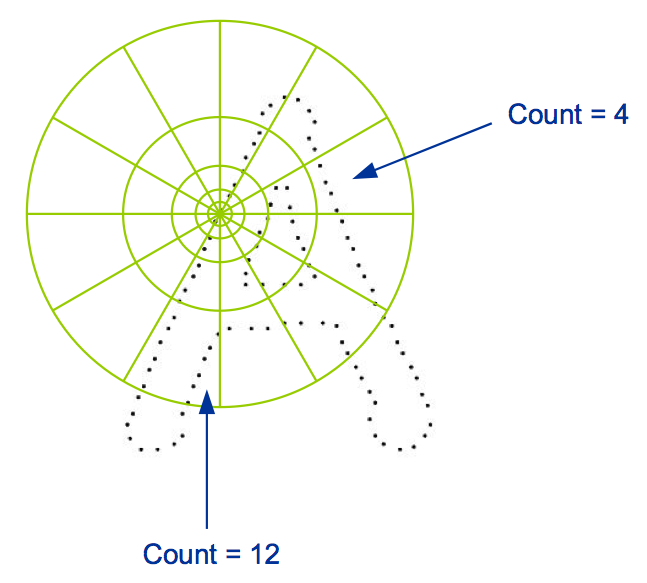
\includegraphics[height=4cm]{IDSC/a-log}
    \caption{对数极坐标系}
    \label{fig:a-log}
  \end{minipage}\hfill
  \begin{minipage}{0.5\textwidth}
    \centering
    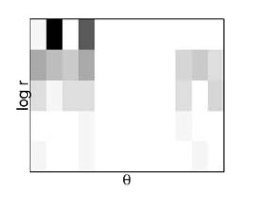
\includegraphics[height=3cm]{IDSC/a-his}
    \caption{形状直方图}
    \label{fig:a-his}
  \end{minipage}
  \end{figure}
\item 计算表示目标边缘上所有采样点之间位置关系的形状上下文,得到的所有点的结果构成了对目标物体形状的描述。
\end{enumerate}

在获得两个目标边缘上每一个采样点的形状上下文后,可以计算这两个目标上采样点之间的匹配关系,根据两目标上所有采样点之间的匹配程度可以得到两形状之间的相似程度,具体实现过程如下。

\begin{enumerate}
\item 假设形状$P$上的采样点为$p_i$和形状$Q$上的采样点为$q_j$,根据$C_{ij}=C(p_i,q_j)$可以计算这两点的匹配代价。
  \begin{eqnarray}
  C_{ij} \equiv C(p_{i},q_{j}) = \frac{1}{2}\sum^{n}_{k=1}\frac{[h_{i}(k)-h_{j}(k)]^{2}}{h_{i}(k)+h_{j}(k)}
  \end{eqnarray}
  其中$C_{ij}$为点$p_i$和$q_j$匹配的代价值,$h_{i}(k)$和$h_{j}(k)$表示点$p_i$和$q_j$的形状上下文。若$C_{ij}$值越小,则点$p_i$和$q_j$的形状上下文越相似,这两点的匹配程度越高~\cite{杨小娜2013基于形状上下文的目标形状识别与匹配}。
\item 对两个形状轮廓边缘上的采样点进行匹配时,必须将采样点一一对应,并且使全部点的匹配代价值的和最小,即
  \begin{eqnarray}
  H(\pi) = \sum_{i}C(p_{i},q_{\pi(i)})
  \end{eqnarray}
  其中$\pi$是一种置换,约束条件是实现采样点的一一对应匹配,使用匈牙利算法可以解决。
\item 使用薄板样条(Thin Plate Spline, TPS)模型表示弹性坐标转换。用两个独立的TPS函数来模拟坐标的变换,从第一个形状的任意位置映射到第二个形状。
  \begin{eqnarray}
  T(x,y)=(f_{x}(x,y),f_{y}(x,y))
  \end{eqnarray}
\item 计算两个形状之间的距离:
  \begin{multline}
  D_{sc}(P,Q)=\frac{1}{n}\sum_{p\in P}arg \min_{q\in Q}C(p,T(q))+\\
  \frac{1}{m}\sum_{q\in Q}arg \min_{p\in P}arg \min_{p\in P}C(p,T(q))
  \end{multline}
  其中$T$为形状$Q$上的点到$P$的TPS变换。
\end{enumerate}

内距离形状上下文是在形状上下文的基础上进行改进,即在内距离形状上下文中统计采样点的位置关系时使用内距离代替了形状上下文中的欧式距离。内距离是指目标轮廓上的两点位于其形状内部距离的最短值,如图~\ref{fig:innerdistance}所示。内距离形状上下文相对应形状上下文而言,对目标的非刚性变化更加敏感,描述局部特征具有更好的鲁棒性。
\begin{figure}[H] % use float package if you want it here
  \centering
  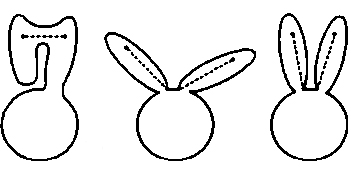
\includegraphics[height=2.5cm]{IDSC/innerdistance}
  \caption{内距离}
  \label{fig:innerdistance}
\end{figure}

在本文研究中使用内距离形状上下文来提取浮游生物的形状特征,主要思想是通过内距离形状上下文计算待识别样本形状与已知浮游生物形状模板之间的相似度来描述形状特征,具体实现过程如下。

\begin{enumerate}
\item 针对每个数据集,选取$n$张不同形状的浮游生物图像,通过人工标注的方法得到这些图像中浮游生物的形状真值图作为形状模板。
\item 采用内距离形状上下文计算数据集中所有浮游生物图像和n张形状模板之间的距离,每张图像都会得到$n$个距离,这些距离表示每张图像的形状与形状模板之间的相似程度。针对每幅图像计算得到的$n$个值可以构成一个$n$维向量,这个向量可以描述该目标形状特征。
\end{enumerate}


\subsubsection{方向梯度直方图}

方向梯度直方图(Histogram of Oriented Gradients, HOG)由Dalal等人在2005年提出~\cite{dalal2005histograms},是一种特征描述方法,具有良好的旋转和平移一致性,被广泛的用于目标检测中。方向梯度直方图的基本思想是通过描述局部区域内的灰度梯度来表示图像的特征,其算法过程如下:

\begin{enumerate}
\item 先将图像进行灰度化,然后采用Gamma校正和灰度归一化处理获得的灰度图像。由于采集的图像受到光照变化、阴影的影响,通过Gamma校正来调节对比度,减少光照等其他因素的影响。

  Gamma压缩公式为:
  \begin{eqnarray}
  I(x,y) = I(x,y)^{gamma}
  \end{eqnarray}
\item 采用梯度算法计算所获得的灰度图像的梯度,获得目标的轮廓信息。

  在计算图像梯度时,通常采用一阶微分模板$[-1,0,1]$求梯度,对图像上任意一点用该模板可以得到垂直和水平方向上的梯度:
  \begin{eqnarray}
  G_{x}(x,y)=H(x+1,y)-H(x-1,y)\\
  G_{y}(x,y)=H(x,y+1)-H(x,y-1)
  \end{eqnarray}

  梯度的幅值和方向计算公式为:
  \begin{eqnarray}
  G(x,y)=\sqrt{G_{x}(x,y)^{2}+G_{y}(x,y)^2}
  \end{eqnarray}
  \begin{eqnarray}
  \theta(x,y)=\tan^{-1}\frac{G_{y}(x,y)}{G_{x}(x,y)}
  \end{eqnarray}

\item 将图像分为Cell(即单元),每个单元都由若干个像素组成。%,如$6 \times 6 \frac{\textrm{像素}}{\textrm{单元}}$。
\item 用直方图对图像中所有单元中的梯度方向加权统计。梯度的范围为0至360度,将其分为n份,统计梯度方向落在每份区域内的梯度加权值。
\item 每几个单元组成一个块(Block),将重叠单元块进行标准化,然后把块中所有单元的直方图向量组合起来得到的向量就是该块的特征描述符。
\item 图像中所有块的特征向量组合到一起就得到了该幅图像的HOG特征。
\end{enumerate}

在本文实验中,使用方向梯度直方图来提取浮游生物的形态特征,在实验中将图像处理为$256 \times 256$,将单元大小设定为$32 \times 32$。

\subsubsection{尺度不变特征变换}

尺度不变特征变换(Scale Invariant feature transform, SIFT)是一种局部特征描述算法,在1999年由Lowe提出\cite{lowe1999object},后来又进行了完善。SIFT有旋转不变和尺度不变等性质,并且被广泛的用于目标识别、目标匹配等领域中。SIFT算法的基本思想是提取图像中的高健壮性的特征点,通过对这些特征点的描述实现对图像中目标特征的描述,该算法的基本实现如下:

\begin{enumerate}
\item 采用高斯函数和图像下采样构建多尺度空间。

  将原图像与不同参数的高斯函数卷积可以实现在不同尺度下对图像滤波:
  \begin{eqnarray}
  L(x,y,\sigma) = G(x,y,\sigma) \ast I(x,y)
  \end{eqnarray}
  其中$I(x,y)$表示原始图像,$L(x,y,\sigma)$表示滤波后得到的图像,$G(x,y,\sigma)$表示高斯函数,
  \begin{eqnarray}
  G(x,y,\sigma)=\frac{1}{2\pi \sigma^{2}}e^{-\frac{x^{2}+y^{2}}{2\sigma^{2}}}
  \end{eqnarray}
  上式中$x,y$是空间坐标,参数$\sigma$决定着对图像滤波程度。为了有效的确定图像中的关键点,将图像与两个相邻尺度高斯函数的卷积结果做差,从而构建高斯差分尺度空间(DOG):
  \begin{multline}
  D(x,y,\sigma)=(G(x,y,k\sigma)-G(x,y,\sigma))\ast I(x,y) \\
  = L(x,y,k\sigma)-L(x,y,\sigma)
  \end{multline}

  采用以上方法来建立图像金字塔。图~\ref{fig:dog}为图像金字塔的结构,从中可以看出每个金字塔包括i个子八度(Octave),并且每个子八度有包括s层。子八度是通过对图像下采样得到i个不同大小的图像(即不同尺度的图像,每次采样得到的图像都为原图的四分之一)组成的。每个子八度中的s(通常为3至5)层是使用高斯函数对图像进行不同程度滤波得到的。
  \begin{figure}[H] % use float package if you want it here
  \centering
  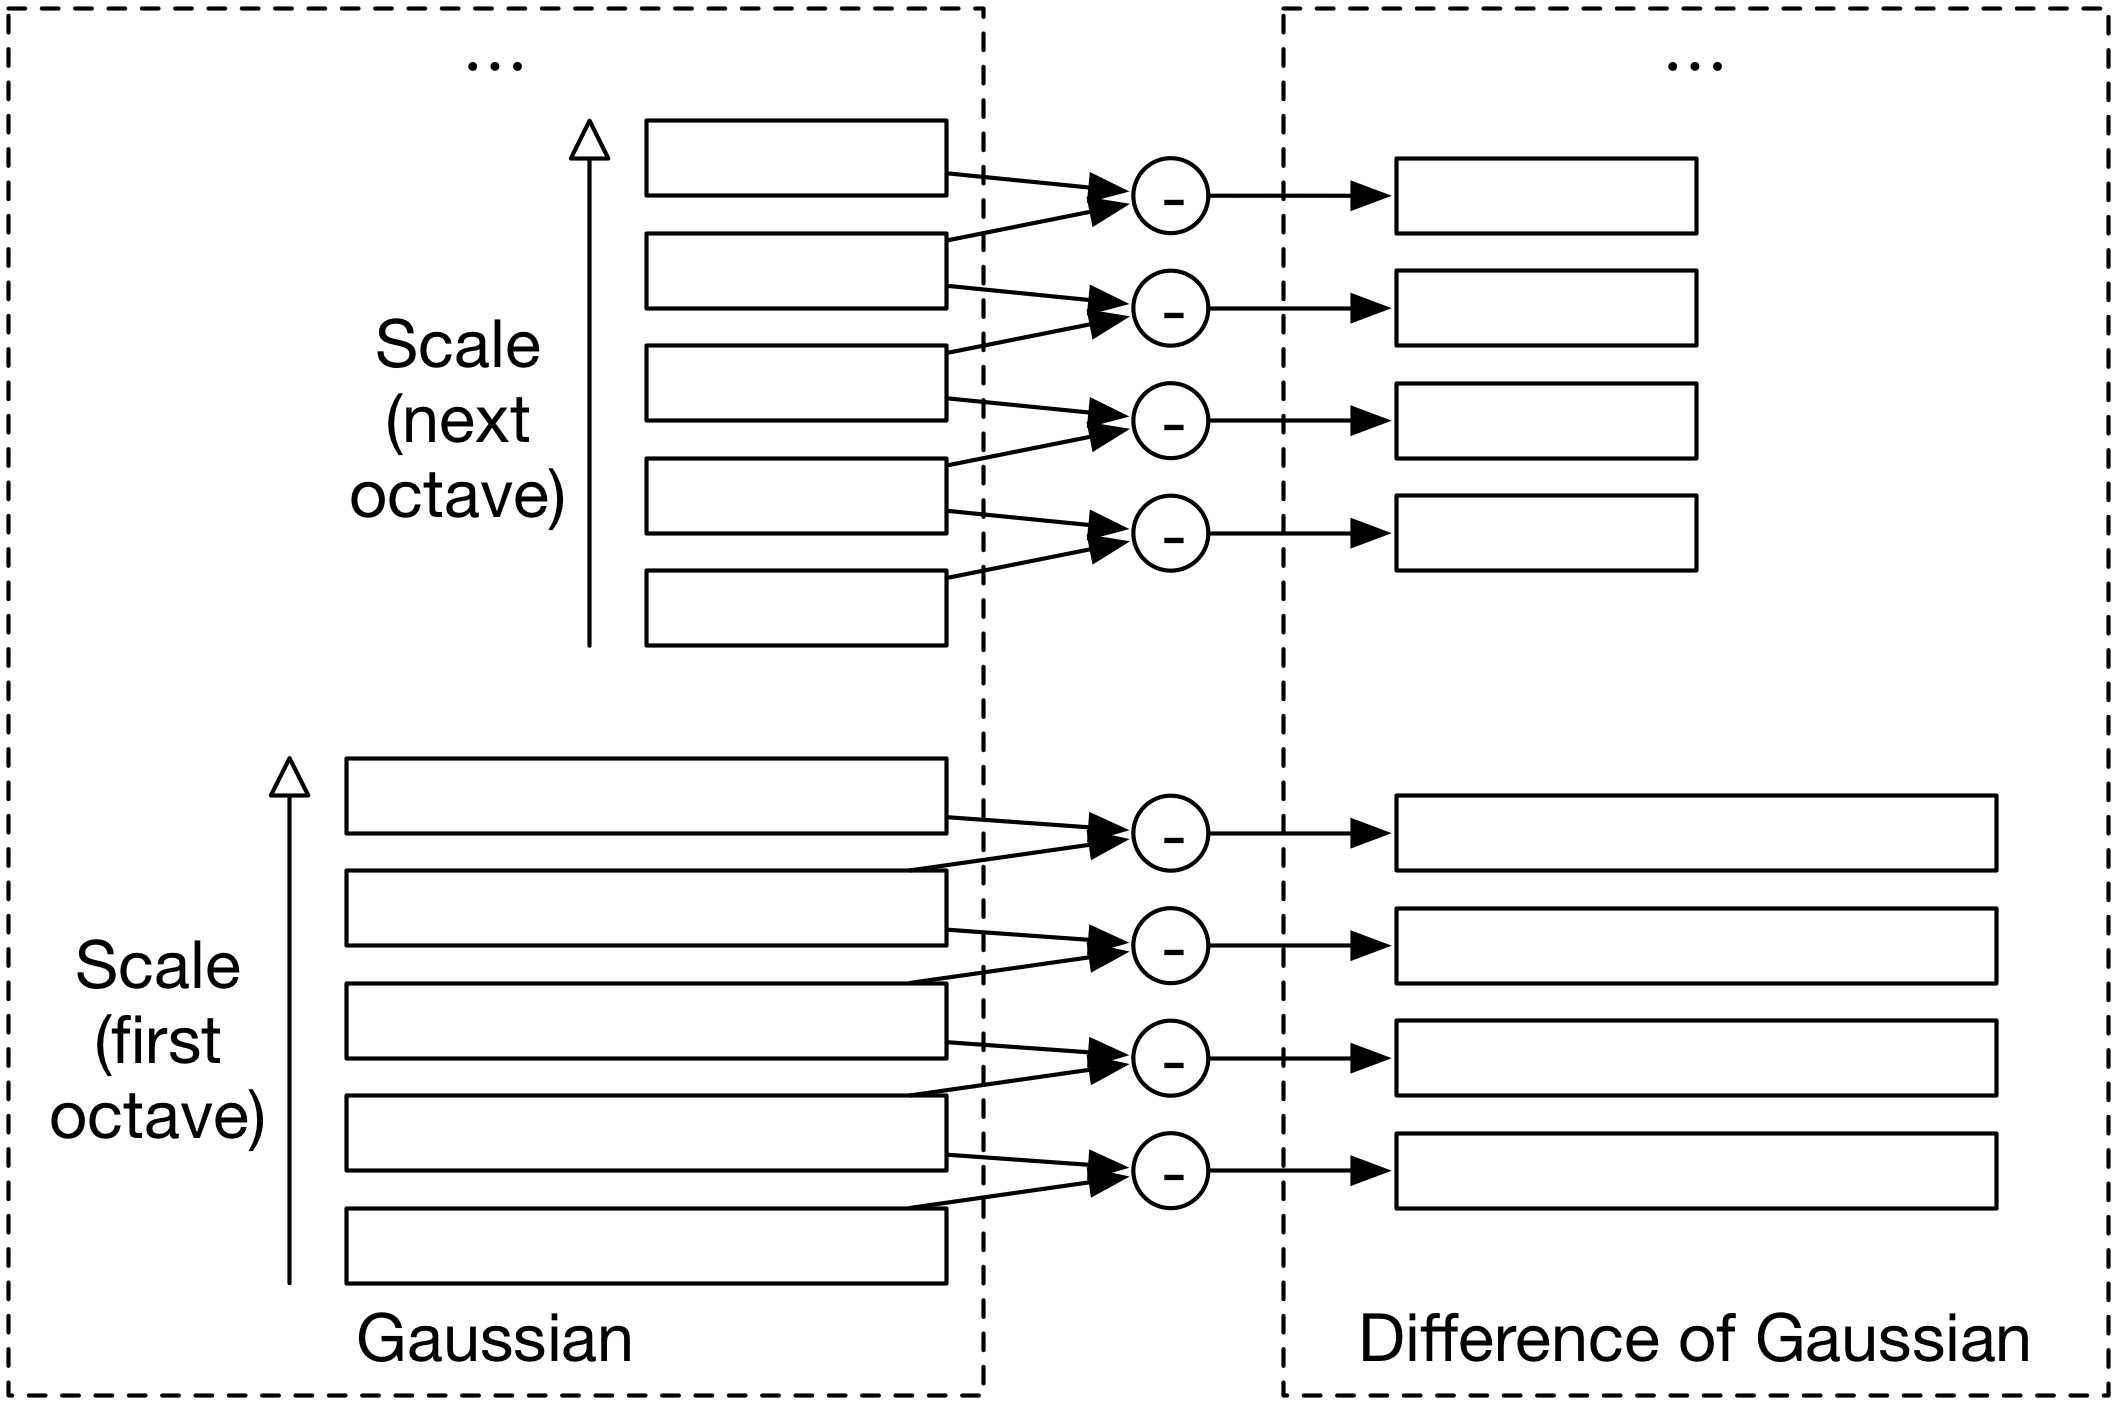
\includegraphics[height=6cm]{sift/DOG}
  \caption{图像金字塔}
  \label{fig:dog}
  \end{figure}

\item 确定图像中的极值点。在DOG空间中确定极值点时,将每一个点与其空间中的邻域比较,观察该点是否是其邻域中的最大值或最小值点。如图~\ref{fig:neg}所示,每一个点的邻域包括其所在层的8邻域以及上下两层的9邻域,所以在确定极值点时每个点要与其空间邻域中的26个相邻点比较。
  \begin{figure}[H] % use float package if you want it here
  \centering
  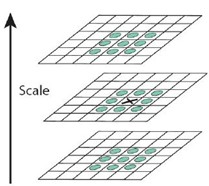
\includegraphics[height=4cm]{sift/neg}
  \caption{检测尺度空间的极值点}
  \label{fig:neg}
  \end{figure}
\item 精确定位特征点。得到的极值点中会存在着一些对比度较低和边缘响应点,将它们去除后保留下来的点就是特征点,即关键点。

  在对关键点的位置和尺度进行精确定位时,采用拟和三维二次函数将关键点中对比度较低的点和边缘相应点去除,从而增强特征描述的稳定性和抗噪能力,实现过程如下。

  尺度空间的泰勒展开式如下:
  \begin{eqnarray}
  D(x)=D+\frac{\partial D^{T}}{\partial x}x+\frac{1}{2}x^{T}\frac{\partial^{2}D}{\partial x^{2}}x
  \end{eqnarray}
  对上式中$x$求导,且让导数为零可得到:
  \begin{eqnarray}
  \hat{x} = -\frac{\partial^{2}D^{-1}}{\partial x^{2}}\frac{\partial D}{\partial x}
  \end{eqnarray}
  将上式代入$D(x)$得:
  \begin{eqnarray}
  D(\hat{x})=D+\frac{1}{2}\frac{\partial D^{T}}{\partial x}\hat{x}
  \end{eqnarray}
  若$|D(\hat{x})| \ge 0.03$,则该关键点保留,否则将其去掉。

  另外还要排除图像中边缘上的关键点,位于图像横跨边缘处的关键点主曲率较大,而在竖直边缘处点的主曲率较小~\cite{陈健斌2012图像特征提取及其相似度的研究和实现},通过这一性质来排除无用的关键点。主曲率可以通过Hessian矩阵求得:
  \begin{eqnarray}
  H=\left[ \begin{array}{ll} D_{xx} & D_{xy}\\ D_{xy} & D_{yy} \end{array} \right]
  \end{eqnarray}
  若H的特征值为$\alpha, \beta$,其中$\alpha$较大,$\beta$较小,则
  \begin{eqnarray}
  Tr(H)=D_{xx}+D_{yy}=\alpha + \beta\\
  Det(H)=D_{xx}D_{yy}-(D_{xy})^{2}=\alpha\beta
  \end{eqnarray}
  因此,令$\alpha = \lambda\beta$,则:
  \begin{eqnarray}
  \frac{Tr(H)^{2}}{Det(H)}=\frac{(\alpha+\beta)^{2}}{\alpha\beta}=\frac{(\gamma\beta+\beta)^{2}}{\gamma\beta^{2}}=\frac{(\gamma+1)^{2}}{\gamma}
  \end{eqnarray}

\item 确定关键点方向参数。在得到图像中关键点后,为了使其具有旋转不变性,需要确定它们的主方向。若关键点邻域内其他像素点$(x,y)$的梯度幅值和方向如下:
  \begin{eqnarray}
  m(x,y)=\sqrt{(L(x+1,y)-L(x-1,y))^{2}+(L(x,y+1)-L(x,y-1))^{2}}
  \end{eqnarray}
  \begin{eqnarray}
  \theta(x,y)=\tan 2\frac{L(x,y+1)-L(x,y-1)}{L(x+1,y)-L(x-1,y)}
  \end{eqnarray}

  用直方图对关键点相邻区域内所有像素点的梯度方向进行统计,其横坐标的范围为0至360度。关键点的方向就是梯度直方图的峰值所表示的梯度方向。
\item 对关键点进行描述。在确定完关键点方向后,以关键点方向为轴建立坐标系生成关键点的特征描述子,具体过程如下:
  \begin{enumerate}
  \item 首先,将关键点作为中心点,取其$16\times16$邻域,然后计算其中所有像素点的梯度。
  \item 将这个邻域分为16个$4\times4$的子区域,用8个bin的直方图加权统计每个子区域内像素的梯度方向。
  \item 将得到的所有直方图结合在一起可以得到一个128($16 \times 8$)维的向量,该向量就是对关键点的特征描述。
  \end{enumerate}
\end{enumerate}

SIFT算法通过提取并描述图像中的关键点来表示图像的特征。SIFT对不同图像提取得到的关键点数量是不同的,每幅图可能包含成百上千个。因此,在进行目标识别过程中,采用SIFT特征来描述每幅图像时得到特征向量数量各不相同,特征点数量越多特征向量越多,分类计算量也越大。因此,用SIFT算法进行图像分类时通常要用到Bag of Words模型。

Bag of Words模型也称为“词袋”,最初用于文本分类中,基本思想是假设两个文本,不考虑其中的语法、词序等,把文本看成一系列词汇的组合,将构成这两个文本的所有词汇放在一起,得到一个词袋,然后这两个文本又可以用这个词袋中的词汇重新描述。同理,将SIFT算法用于目标识别时,每幅图像可以看成一个文本,描述图像中每个特征点的特征向量看做为词汇,将所有图像中所有特征点的特征向量放在一起构成一个词袋,然后用这个词袋重新对每幅图像的特征进行描述。这样得到的描述每幅图像的特征向量不仅规整,而且减少了计算量,大大提高了计算效率。使用BOW模型描述图像特征的基本步骤如下:
\begin{enumerate}
\item 若数据集中有n张图像,采用SIFT算法提取所有图像中的特征点,并得到每一个特征点的128维特征向量。
\item 将SIFT提取的n张图像的所有特征点放在一起,采用K-means对这些特征点聚类,假设一共聚为m类。
\item 每个类别分别有一个聚类中心,计算每幅图像中所有特征点到这m个中心的距离,将每个特征点分别归到距其最近中心所属的类别中去,可以使用直方图向量统计每幅图像中特征点在m个类别中出现频率,该向量就是对图像特征的描述。
\end{enumerate}

在本文研究中,采用SIFT提取数据集中全部图像的特征点,然后用K-means算法将所有特征点聚为100类,分别描述每幅图像中特征在100类中出现的频率,因此每幅图像的特征可以得到一个100维的特征向量。

\section{浮游生物特征选择}
\label{sec:featureselection}

特征选择是指去除特征中的冗余部分,降低特征维数,保留有用的特征,同时提高分类的效率和准确率。在分类识别中,有效的特征信息是训练优秀分类器的重要因素,特征中的冗余部分不仅会影响分类的结果~\cite{姚旭2012特征选择方法综述},还会降低效率,因此在机器学习过程中对特征进行选择是至关重要的。

到目前为止,已经有很多研究者对特征选进行研究定义:在1992年Kria和Rendell~\cite{Kira1992The}提出特征选择是找到可以对目标进行识别的最小特征集合;后来John等人~\cite{John1998Irrelevant}提出减少特征维数是在能够提高或不要降低准确率的前提下进行;Koller等人~\cite{Koller2000Toward}认为在选择最小的特征集合时确保分类结果的分布与原始类分布相似;后来Dash等人\cite{Dash1997Feature}结合上述观点,将特征选择定义为在不降低分类准确度且不改变类比分布的情况下保留尽可能小的特征集合。

特征选择方法的基本步骤是:先生成候选的特征子集,然后对其进行评价,判断选择结果是否符合停止准则,若符合则对检验结果,否则重新生成候选特征子集。目前特征选择的方法有很多,按照搜索测量和评价标准的不同将其分类。

\subsection{按搜索测量进行特征选择的方法}

根据特征选择方法在选取子集时使用的搜索策略将其分为:全局最优、随机搜索和启发式搜索,下面对这三种方法分别进行介绍。

\subsubsection{基于全局最优搜索策略的特征选择方法}

分支界定是基于全局最优搜索策略的特征选择方法中可以获得最优结果的唯一算法~\cite{姚旭2012特征选择方法综述},该算法的基本思想是:将所有可能的特征选择组合构成一个树状结构,按照特定的规则对树进行搜索,使搜索过程尽可能得到最优解而不必须遍历整个树。使用这种方法的前提是需要准则判据对特征有单调性,但是在处理高纬度特征时,该算法的时间复杂度较高。所以,基于全局最优搜索策略的算法虽然可以获得最优结果,但是很难被广泛的使用。

\subsubsection{基于随机搜索策略的特征选择方法}

基于随机搜索策略的特征选择方法通过有一定智能的随机搜索策略实现,在计算过程中该方法结合了特征选择与粒子群优化算法、模拟退火算法、遗传算法等,将采样和概率推理看做选择的基本,按照每个特征分类时的有效性,给它们分别赋予一个权值,然后按照设定或自适应阈值确定对分类有用的特征。若某个特征的权重超过该阈值,则这个特征便是有用的~\cite{宁永鹏2014高维小样本数据的特征选择研究及其稳定性分析}。

\subsubsection{基于启发式搜索策略的特征选择方法}

利用问题的启发信息作为引导,并进行搜索的方法称为启发式搜索,该方法可以降低问题的复杂度,并且减少搜索的范围。在特征选择过程中全局最优的搜索算法计算量可能很大,因此出现了以启发式搜索策略为基础的特征选择算法,该方法可以分为以下几种:单独最优特征组合、浮动搜索、增l去r选择方法、序列前向选择方法、广义序列前向选择方法、序列后向选择方法、广义序列后向选择方法、广义增l去r选择方法。虽然启发式搜索策略的效率较高,但是是以牺牲全局最优为代价。

\subsection{按评价准则进行特征选择的方法}

在特征选择过程中,对所选择特征好坏的有不同的评价方法。根据评价方法是否依赖于后续的学习算法能够将特征选择方法分为两种:过滤式(Filter)和封装式(Wrapper)~\cite{宁永鹏2014高维小样本数据的特征选择研究及其稳定性分析}。过滤式特征选择独立于之后的学习算法,通常情况下可以直接使用训练数据的统计性能对特征进行评估,虽然计算效率较高,但是之后使用学习算法得到的结果和评估结果可能相差较大。封装式方法需要用后续的学习算法来对特征子集进行评价,因此结果与之后学习算法相差较小,但是计算量大。下面分别介绍这两种方法。

\subsubsection{过滤式评价准则的特征选择方法}

过滤式特征选择具有较高的效率,该方法通常用评价准则来增加特征与类别之间的相关性,去除掉不相关的杂质特征,优化特征子集,就像过滤器一样。根据评价准则可以将过滤式方法分成:一致性度量、依赖性度量、信息度量以及距离度量。这些方法的一个主要问题在找到的最优特征子集的规模往往较大,其中会包含一些噪声,但计算效率较高。

\subsubsection{封装式评价准则的特征选择方法}

封装式方法需要用之后的学习算法对选取的特征进行评估,将学习算法看做特征选择的一部分,按照学习得到的分类器性能进行特征选择。采用封装式方法进行特征选择时,用选取的特征集合来训练分类器,获得分类器的分类准确率可以作为评价所选特征重要性的标准。基于封装式的特征选择方法的计算速度要比基于过滤式的方法慢,但是它选择得到的特征子集维数较小,如今该方法在特征选择领域有较为广泛的应用。

在本文实验中,由于提取的图像特征种类丰富并且维数较高,因此其中会包含部分的冗余特征,这些特征不仅不利于分类准确率的提高,还降低了计算效率,因此在特征提取后又进一步进行了特征选择,采用的特征选择算法为基于封装式评价准则的特征选择算法。

\section{本章小结}

浮游生物种类繁多,类别相近的生物之间形态特征相差较小,而浮游植物和动物之间的差异又较大,这些特点增加了浮游生物分类的难度,因此需要全面充足的特征信息对浮游生物的形态特征进行描述。本章介绍了根据浮游生物形态特征选用的特征提取方法,包括:几何灰度统计特征;局部二值模式、二元梯度轮廓、Gabor滤波器等纹理特征描述算法;内距离形状上下文、尺度不变特征变换等局部特征描述算法。这些特征提取算法可以对浮游生物的大小、形状、灰度、纹理等信息全面的描述。

由于提取的浮游生物特征较多,在提取的特征中可能存在冗余或不相关的信息,这些信息的存在不利于分类性能和准确率的提高,因此我们引入了基于封装式评价准则的特征选择方法对提取的特征进行筛选,去除冗余信息,降低维数,进而可以提高的分类器的泛化能力和整体性能。










